\chapter{Discussion}
%In this section you discuss any issues that came up while developing
%the system.  If you found something particularly interesting,
%difficult, or an important learning experience, put it here.  This is
%also a good place to put additional figures and data.
Mean Absolute Percentage Error (MAPE) does not tell the whole story of a model's performance. The true measure of performance is how useful the model output is to energy producers. The model's confidence in a prediction is almost as important as the accuracy of the prediction and the total energy produced over the day matters.
The forecast downward shortwave irradiance, the largest factor in measured irradiance, rarely drops. It is almost exclusively on very high variance days that it deviates from a sine wave. The downward diffuse shortwave irradiance, the other network input data value, is a much smaller part of the total irradiance and has, to the bare eye, seemingly no correlation with the observation values. Despite this, the models show generally fantastic performance in predicting the irradiance.
The full model was able to utilize the forecast data from the surrounding area to achieve noticeably better performance. Of course, since the limited model uses only one-ninth of the data of the full model, some hyperparameter tuning had to be done to optimize its performance and some of the performance difference could be explained by worse optimization.
With the data at hand, it is not possible to separate the performance of the weather forecast model producing our input data and the performance of our models. We do not know how close this model comes to maximizing the information available in the input data.

Fig.~\ref{fig:disc_low} shows side-by-side the two models' performance for the same calm day. The full model was able to track the observations more closely with more confidence. This was typical for all calm days.
\begin{figure}[ht!]
    \centering
    \subfloat[Full model]{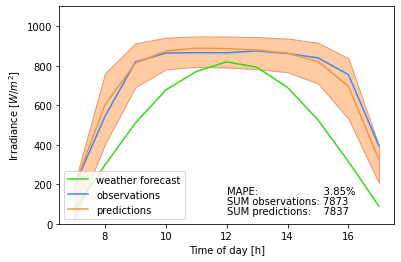
\includegraphics[scale=0.5]{imgs/graphs/disc/disc_med_full.png}}\qquad
    \subfloat[Limited model]{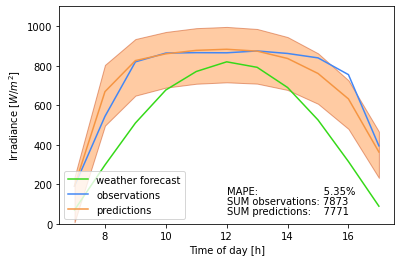
\includegraphics[scale=0.5]{imgs/graphs/less/low/low_g_1.png}}\qquad
    \caption{Comparison of model performance on a clear day.
    \label{fig:disc_low}}
\end{figure}

In Fig.~\ref{fig:disc_med} we can see a comparison between the two models on a less predictable day. Again, the full model shows better performance in tracking, primarily because the limited model misses an end-of-day prediction. There are similar days where the limited model shows slightly better performance.
\begin{figure}[ht!]
    \centering
    \subfloat[Full model]{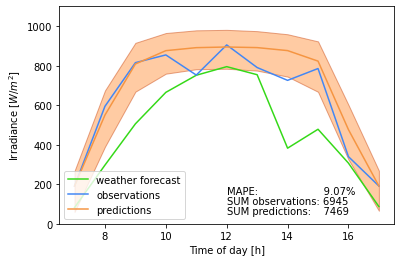
\includegraphics[scale=0.5]{imgs/graphs/full/medium/med_g_3.png}}\qquad
    \subfloat[Limited model]{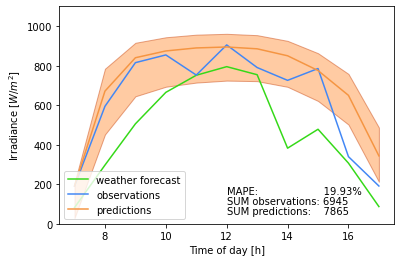
\includegraphics[scale=0.5]{imgs/graphs/less/medium/med_g_1.png}}\qquad
    \caption{Comparison of model performance on a day with some drops in irradiance.
    \label{fig:disc_med}}
\end{figure}

Fig.~\ref{fig:disc_high} shows a clear example of the performance difference between the models on erratic days. The full model, while still having a high error gets somewhat close to keeping the observations within its much smaller 90\% confidence interval than the limited model. The limited model also predicts much more irradiance over the day than the, already too high, full model.
\begin{figure}[ht!]
    \centering
    \subfloat[Full model]{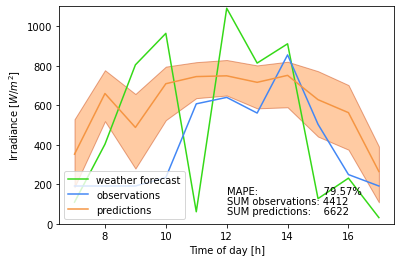
\includegraphics[scale=0.5]{imgs/graphs/full/high/high_3.png}}\qquad
    \subfloat[Limited model]{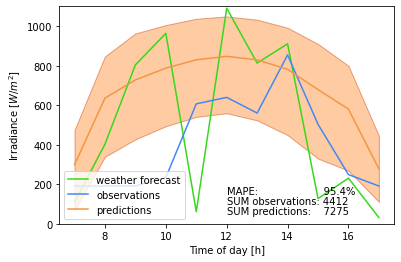
\includegraphics[scale=0.5]{imgs/graphs/less/high/high_4.png}}\qquad
    \caption{Comparison of model performance on an erratic day.
    \label{fig:disc_high}}
\end{figure}



\section{Limitations and Future Work}
We used a dataset of a fairly limited size, only 425 days. A few years of data for training the model would likely yield somewhat better results. The data can be processed more before being input into the network to account for known variables like daily and yearly swings in irradiance, which might improve performance. There exists satellite irradiance measurement data that might be used for improving accuracy. It would be interesting to see if a neural network could extract information from the seven pyranometers scattered across the power station, rather than only dropping the highest and lowest values and taking an average. 

The model also has huge potential in utilizing more varied data in addition to a larger time span, other exogenous data that might further help relate the input forecast to the actual irradiance. Experimenting with wind data, both historical and forecast data, may well unlock further steps in performance.

Sadly, there is not a standard benchmark for solar irradiance forecast models, and the data used by others who have done similar work is not available, so we can't make a proper comparison between methodologies and models. 

\section{Conclusion\label{sec:conclusions}}
The results clearly show that relying on forecast irradiance data from meteorological models is a very effective, but not perfect, method of accurately predicting irradiance in a single area. A transformer model, the Temporal Fusion Transformer, managed to very effectively translate patterns in meteorological irradiance forecasts to accurate local irradiance predictions utilizing spatially and temporally adjacent data.\\
%%% Local Variables: 
%%% mode: latex
%%% TeX-master: "DEGREE-NAME-YEAR"
%%% End: 
